\chapter{CONCEITOS FUNDAMENTAIS} \label{conceitos}

\begin{comment}
\emph{Questão a ser respondida pelos Conceitos: Quais são os fundamentos teóricos relevantes?}
Aqui define-se os principais termos e conceitos que serão utilizados ao longo do trabalho. Para essa seção é recomendada a utilização de livros e artigos já consolidados na literatura. Todos os parágrafos dessa seção devem ter pelo menos uma citação. 
\end{comment}

Para o entendimento de alguns softwares e o porquê de estarem sendo utilizados, existem alguns conceitos que devem ser compreendidos para o total entendimento do projeto. Estes conceitos são:

\textbf{Conteinerização:} Uma forma de virtualização feita para ser mais rápida e flexível que a emulação, é um processo de implantação que consegue ser executado em diversos dispositivos e sistemas operacionais, isso ocorre pelo fato de que um contêiner consegue armazenar os arquivos e bibliotecas para ser executado, permitindo um usuário executar uma aplicação de outro sistema operacional no sistema operacional que o mesmo possua, além disso, o contêiner permite que falhas ocorram sem afetar outros processos que não estão agrupados no mesmo. \cite{Wen2023}

\begin{comment}
    \textbf{Conteinerização:} Uma forma de virtualização feita para ser mais rápida e flexível que emulação, mas ainda ter sua consistência e isolamento do Sistema Operacional principal \cite{Wen2023}.

    A conteinerização é um processo de implantação de software que agrupa o código de uma aplicação com todos os arquivos e bibliotecas de que ela precisa para ser executado em qualquer infraestrutura. Tradicionalmente, para executar qualquer aplicação em seu computador, era necessário instalar a versão que correspondia ao sistema operacional da sua máquina. Por exemplo, você precisava instalar a versão Windows de um pacote de software em uma máquina Windows. No entanto, com a conteinerização, você pode criar um único pacote de software, ou contêiner, que é executado em todos os tipos de dispositivos e sistemas operacionais. 
\end{comment}

\textbf{Meta-sistema operacional:} Um meta-sistema operacional se trata de um sistema operacional para robôs, o mesmo realiza todas as funções que um sistema operacional faz. O mesmo possui bibliotecas e ferramentas que executam códigos em multiplos computadores. Este sistema operacional é utilizado em robôs...
%https://wiki.ros.org/ROS/Introduction

\begin{comment}
    \textbf{Meta-sistema operacional:} É um sistema operacional que é desenvolvido e executado em outro sistema operacional, permitindo que diferentes processos possam se comunicar durante a execução. Este conceito é aplicado para o ROS.

     It also provides tools and libraries for obtaining, building, writing, and running code across multiple computers. ROS is similar in some respects to 'robot frameworks,' such as Player, YARP, Orocos, CARMEN, Orca, MOOS, and Microsoft Robotics Studio.
\end{comment}
%https://stackoverflow.com/questions/15150599/what-is-the-difference-between-operating-system-and-meta-operating-system#:~:text=The%20basic%20difference%20is%20that,with%20each%20other%20at%20runtime.

\textbf{Middleware:} Uma camada de software que conecta as aplicações a um sistema operacional, permitindo uma comunicação e compartilhamento de dados mais simples entre os componentes de um sistema, esta facilidade permite que os desenvolvedores foquem no desenvolvimento das principais funções de uma aplicação, pois a comunicação entre a aplicação e o sistema operacional está sendo feita pelo middleware.
%Middleware é uma camada de software que conecta o sistema operacional a aplicações, dados e usuários. Ele disponibiliza serviços e recursos compartilhados, como single sign-on (SSO) e gerenciamento de interfaces de programação de aplicações (APIs). Os desenvolvedores podem contar com o middleware para fornecer integrações consistentes e simplificadas entre os componentes da aplicação. Assim, os profissionais podem se concentrar na criação de funcionalidades essenciais, no tempo em que estariam conectando essas funções a diferentes endpoints e ambientes, como sistemas legados.

\textbf{DDS:} Um protocolo middleware e uma API para conexão centrada em dados, este protocolo integra os componentes de um sistema que muitas aplicações precisam, como arquitetura escalar, confiabilidade e prover conectividade de dados de baixa latência. Este protocolo foi criado pela OMG.
%https://www.dds-foundation.org/what-is-dds-3/
%The OMG Data Distribution Service (DDS™) is a middleware protocol and API standard for data-centric connectivity from the Object Management Group® (OMG®). It integrates the components of a system together, providing low-latency data connectivity, extreme reliability, and a scalable architecture that business and mission-critical Internet of Things (IoT) applications need.

%In a distributed system, middleware is the software layer that lies between the operating system and applications. It enables the various components of a system to more easily communicate and share data. It simplifies the development of distributed systems by letting software developers focus on the specific purpose of their applications rather than the mechanics of passing information between applications and systems.

\subsection{FERRAMENTAS}
Para o desenvolvimento do projeto, serão utilizados softwares e ferramentas para que os testes possam ser realizados e analisados. As ferramentas utilizadas serão:

\textbf{Docker:} É uma plataforma utilizada para desenvolvimento, envio e funcionamento de aplicações de maneira separada da infraestrutura por conta da conteinerização, por conta deste fator o usuário consegue gerir as aplicações da mesma maneira que gera sua infraestrutura, outro fator importante é que o Docker permite que as aplicações desenvolvidas sejam testadas e executadas com menos atraso do que a maneira convencional. Contêineres são bons para fluxos de integrações e entregas de trabalho contínuas.\cite{dck2025}
 %Docker is an open platform for developing, shipping, and running applications. Docker enables you to separate your applications from your infrastructure so you can deliver software quickly. With Docker, you can manage your infrastructure in the same ways you manage your applications. By taking advantage of Docker's methodologies for shipping, testing, and deploying code, you can significantly reduce the delay between writing code and running it in production.
%(Fast, consistent delivery of your applications) Docker streamlines the development lifecycle by allowing developers to work in standardized environments using local containers which provide your applications and services. Containers are great for continuous integration and continuous delivery (CI/CD) workflows.
%\newpage

\textbf{ROS2(Robot Operating System 2):} É um meta-sistema operacional de código aberto utilizado para auxiliar a desenvolver aplicações para robôs, o mesmo possui serviços que outros sistemas operacionais normalmente possuem, mas com o foco maior para a área da robótica, facilitando comunicação entre processos, funções que se comunicam com as demais e entre muitos outros. Para o desenvolvimento do projeto, será utilizado o ROS 2 que mantém o conceito modular e distribuido, mas possui melhorias e mais funcionalidades que o ROS original (Observar figura \ref{fig:ROS25}) \cite{ros2025}

%The Robot Operating System (ROS) is a set of software libraries and tools that help you build robot applications. From drivers to state-of-the-art algorithms, and with powerful developer tools, ROS has what you need for your next robotics project. And it's all open source.

%https://wiki.ros.org/ROS/Introduction
%ROS is an open-source, meta-operating system for your robot. It provides the services you would expect from an operating system, including hardware abstraction, low-level device control, implementation of commonly-used functionality, message-passing between processes, and package management. It also provides tools and libraries for obtaining, building, writing, and running code across multiple computers. ROS is similar in some respects to 'robot frameworks,' such as Player, YARP, Orocos, CARMEN, Orca, MOOS, and Microsoft Robotics Studio.
\textbf{Gazebo Simulator:} É um software usado para desenvolver simulações, possui diversos projetos de código aberto para que os interessados possam utilizar e desenvolver suas próprias simulações. Neste software estão presentes também diversos modelos, tanto como objetos como também robôs.(Observar figura \ref{fig:gzb25}) \cite{gzb2025}


% https://gazebosim.org/home Gazebo é uma coleção de bibliotecas de software de código aberto projetadas para simplificar o desenvolvimento de aplicações de alto desempenho. O público-alvo do Gazebo são desenvolvedores, designers e educadores de robôs. No entanto, o Gazebo foi estruturado para atender a diversos casos de uso. Cada biblioteca dentro do Gazebo possui dependências mínimas, permitindo que sejam usadas em tarefas que vão desde a resolução de transformações matemáticas até a codificação de vídeo, simulação e gerenciamento de processos. Basta escolher as bibliotecas necessárias para sua aplicação sem se comprometer com um ecossistema inteiro.
\textbf{TurtleBot3 Burger:} É um robô customizável de preço acessível ao público baseado no modelo ROS para ser utilizado como um material educativo, de pesquisas, entretenimento pessoal e etc, é um robô que foi desenvolvido com o intuito de ser barato, por conta disto, o mesmo não possui uma grande funcionalidade ou qualidade, mas o mesmo compensa na relação da quantidade de aplicações que o mesmo consegue realizar.(Observar figura \ref{fig:tbt3b25}) \cite{turtlebot3_manual}

\textbf{Fast DDS:} Implementação de DDS feita em c++, possui uma biblioteca que oferece uma API e protocolo de comunicação que disponibiliza um modelo Publisher-Subscriber centrado em dados (DCPS). Este modelo visa ser eficiente e confiável para distribuir as informações para o sistema em tempo real.
%https://fast-dds.docs.eprosima.com/en/stable/02-formalia/titlepage.html#
%eProsima Fast DDS is a C++ implementation of the DDS (Data Distribution Service) Specification, a protocol defined by the Object Management Group (OMG). The eProsima Fast DDS library provides both an Application Programming Interface (API) and a communication protocol that deploy a Data-Centric Publisher-Subscriber (DCPS) model, with the purpose of establishing efficient and reliable information distribution among Real-Time Systems.


\textbf{Cyclone DDS:} Implementação de DDS com alto desempenho, permite que os desenvolvedores que o utilizam possam criar "gêmeos" digitais das entidades de seus sistemas permitindo compartilhar estados, eventos, fluxos de dados e mensagens pela rede em tempo real, visa ser rápido, consistente e seguro.
%https://cyclonedds.io/
%Building Portable & Interoperable Distributed Datacentric Systems Cyclone DDS is a high performing, OMG-DDS standard based data sharing technology which allows system designers to create digital twins of their systems' entities to share their states, events, data-streams and messages on the network in real-time and fault-tolerant way.

%TurtleBot is a low-cost, personal robot kit with open-source software. TurtleBot was created at Willow Garage by Melonee Wise and Tully Foote in November 2010. With TurtleBot, you’ll be able to build a robot that can drive around your house, see in 3D, and have enough horsepower to create exciting applications.
%The TurtleBot kit consists of a mobile base, 2D/3D distance sensor, laptop computer or SBC(Single Board Computer), and the TurtleBot mounting hardware kit. In addition to the TurtleBot kit, users can download the TurtleBot SDK from the ROS wiki. TurtleBot is designed to be easy to buy, build, and assemble, using off the shelf consumer products and parts that easily can be created from standard materials. As an entry level mobile robotics platform, TurtleBot has many of the same capabilities of the company’s larger robotics platforms, like PR2.
%TurtleBot3 is made up of modular plates that users can customize the shape. Available in three types: small size Burger and medium size Waffle, Waffle Pi. TurtleBot3 consists of a base, two Dynamixel motors, a 1,800mAh battery pack, a 360 degree LIDAR, a camera(+ RealSense camera for Waffle kit, + Raspberry Pi Camera for Waffle Pi kit), an SBC(single board computer: Raspberry PI 3 and Intel Joule 570x) and a hardware mounting kit attaching everything together and adding future sensors. Turtlebot3 was released on May 2017.



%The TurtleBot3 in specific is a small, affordable, and customizable, ROS-based mobile robot for use in education, research, hobby projects, and product prototyping. The goal of TurtleBot3 is to provide a low cost, highly flexible robotics development platform without having to sacrifice functionality and quality, while at the same time offering enough expandability to fit a wide variety of complex robotics applications. The TurtleBot3 can be customized in various ways using simple mechanical components and through the use of upgraded electronic components including custom computers and sensors. In addition, the TurtleBot3 has continued to evolve it’s out of the box performance by continually upgrading the included cost-effective and small-sized SBC suitable for robust embedded systems. The TurtleBot3’s core technology of SLAM, Navigation and Manipulation makes it suitable for a wide variety of research and service robotics applications.
\begin{figure}[htb]
    \centering
    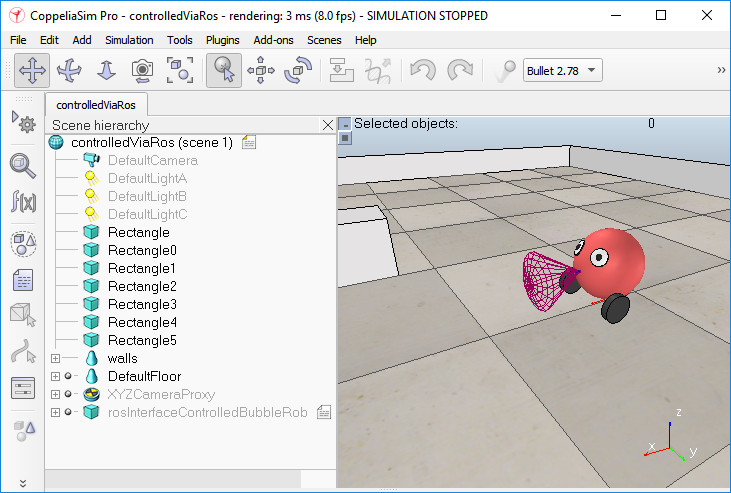
\includegraphics[width=0.5\linewidth]{Figures/ROS.png}
    \caption{TROCAR ESSA IMAGEM \cite{cop2020}}
    \label{fig:ROS25}
\end{figure}

\newpage
\begin{figure}[htb]
    \centering
    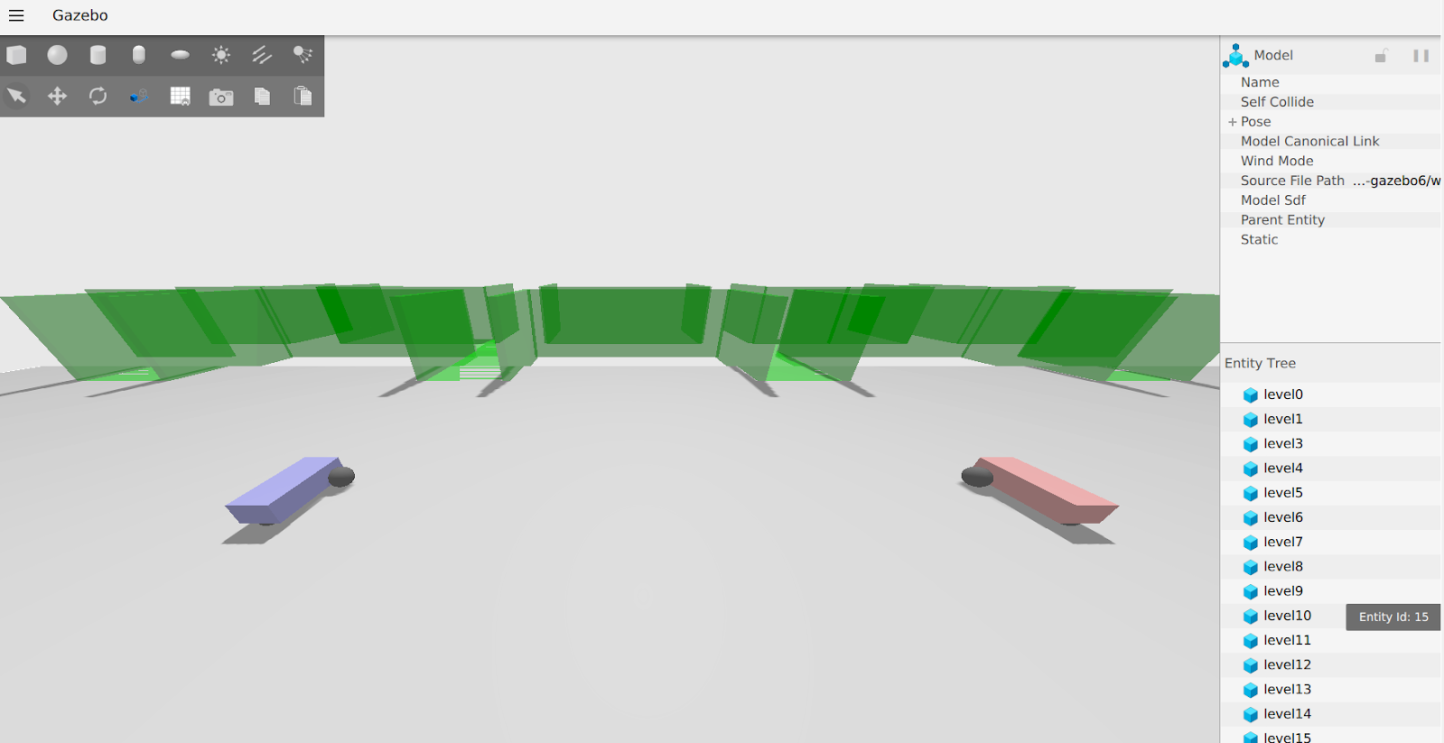
\includegraphics[width=0.5\linewidth]{Figures/gazebo.png}
    \caption{Exemplo utilizando o Gazebo Simulator \cite{gzb2025}}
    \label{fig:gzb25}
\end{figure}

\begin{figure}[htb]
    \centering
    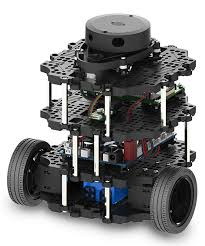
\includegraphics[width=0.3\linewidth]{Figures/TurtleBot3.jpg}
    \caption{TurtleBot3 Burger \cite{tbt2025}}
    \label{fig:tbt3b25}
\end{figure}